\documentclass{beamer}
%\usepackage[dutch]{babel}
\usepackage[utf8]{inputenc}
\usepackage[T1]{fontenc}
\usepackage{amsmath}
\usepackage{amssymb}
\usepackage[makeroom]{cancel}
\usepackage{color}
\newcommand<>{\xxcancel}[1]{\alt#2{\cancel{#1}\vphantom{#1}}{#1}} %has apparently no effect
%\renewcommand{\CancelColor}{blue}

\newcommand{\C}{\ensuremath{\mathbb{C}}}
\newcommand{\N}{\ensuremath{\mathbb{N}}}
\newcommand{\E}{\ensuremath{\mathbb{E}}}
\newcommand{\norm}[1]{\left\|#1\right\|} % commando's met argumenten
\newcommand{\pa}[2]{\frac{\partial #1}{\partial #2}}
\newcommand{\ppa}[2]{\frac{\partial^2 #1}{\partial #2^2}}
\newcommand{\dd}{\ensuremath{\mathrm{d}}}
\newcommand{\U}{\ensuremath{\boldsymbol{\rho}}}
\newcommand{\cts}{\ensuremath{\boldsymbol{\Phi}_T}} %Coarse time step
\newcommand{\V}{\ensuremath{\mathbf{v}}}
\newcommand{\jv}{\ensuremath{\mathbf{\hat{Jv}}}}
\newcommand{\jvpde}{\ensuremath{\mathbf{Jv}_{FP}}}

\begin{document}Problem: $ \texttt{Var}(\jv)  \sim \mathcal{O}(1/(\varepsilon^2  N)) \Rightarrow $    Numerical noise for $ \varepsilon \ll 1$    


 % % % 


\section[Pieter Van Nuffel]{}



\begin{frame}
\frametitle{Pieter Van Nuffel}


\begin{itemize}
\item 2006-2011: Master in Physics and Astronomy (UGent)
	\begin{itemize}
	\item {\textbf{Master thesis}}: Simulation of Information Entropy in Financial Markets with Molecular Dynamics.
	\end{itemize}
\item 2012-2015: Teaching assistent (KU Leuven KULAK)
\item 2015-current: PhD student
	\begin{itemize}
	\item {\textbf{Promotor}}: Giovanni Samaey
	\item {\textbf{Research topics and interests}}: 
	Coarse Bifurcation Analysis of Stochastic Agent-based
	Network Models, Uncertainty Quantification,  Multiscale Methods
	\end{itemize}
\end{itemize}

\end{frame}


\begin{frame}
\frametitle{Fokker-Planck equation}

\begin{equation*}
\label{fokkerplanck}
\pa{\rho(x,t)}{t} + \pa{(a(x) \rho(x,t))}{x} = D  \ppa{\rho(x,t)}{x} 
\end{equation*}
\begin{center}
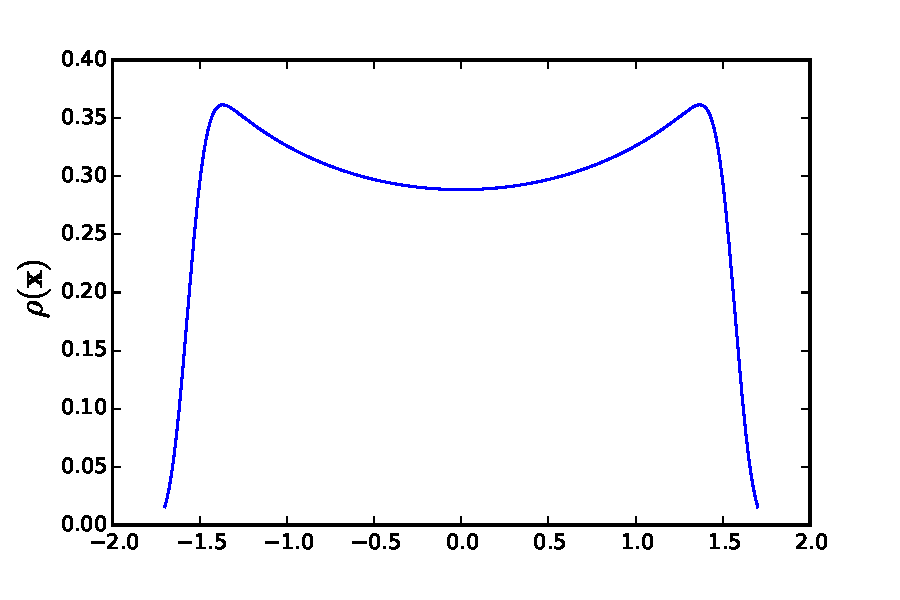
\includegraphics[width=6.5cm]{../Problems/WeightedParticles/checkSystem/plots/rho_pde}
\end{center}


Simulate an ensemble of $N$ particles evolving according to the corresponding SDE
\begin{equation*}
    \dd x = a(x) \dd t + \sqrt{2D} \cdot \dd{W_t}.
\end{equation*}




\end{frame}

\begin{frame}

\frametitle{Coarse time stepper}

\begin{equation*}
\U(t + n \Delta t) = \cts(\U) = (\mathcal{R} \circ \mathcal{E}(n \Delta t, \omega) \circ  \mathcal{L}(\mathbf{\omega})  ) (\U(t))
\end{equation*}


\begin{itemize} [<+->]
\item 
\begin{block} 
{Lifting $\mathcal{L}: \U \rightarrow \mathbf{x}  $}
\end{block}
\item
 \begin{block} {Evolution  $\mathcal{E}$: \\ Simulation of the SDE for $N$ particles over $n$ timesteps. }
\begin{equation*}
   \mathbf{x}^{n + 1} = \mathbf{x}^{n} + a(\mathbf{x}^n) \Delta t +  \sqrt{2D \Delta t}\cdot \boldsymbol{\xi}^n 
\end{equation*}
with \begin{equation*}\xi^n(\omega)  \sim \mathcal{N} (0,1)
\end{equation*}
\end{block}

\item 
\begin{block} {Restriction $\mathcal{R}: \mathbf{x} \rightarrow \U $}
\begin{equation*}
\frac{1}{N} \sum_{i=1}^{N}  w_i \cdot \chi_{\Delta_j}(x_i) = \rho_j  
\end{equation*}
\end{block}

\end{itemize}

\end{frame}


\begin{frame}
\frametitle{Evaluating Jacobian-vector products}
\begin{equation*}
 \U_* - \cts(\U_*) =0
\end{equation*}

\begin{equation*}
\mathbf{Jv} = D(\cts) \cdot \mathbf{v} \approx \frac{\cts (\U + \varepsilon \mathbf{v}, \boldsymbol{\omega_1} )  - \cts (\U, \boldsymbol{\omega_2})}{\varepsilon} 
\end{equation*}

\pause
\begin{block}{Problem: numerical noise for $ \varepsilon \ll 1$ }
Repeating $\cts$ with two sets of random numbers $\boldsymbol{\omega_1},  \boldsymbol{\omega_2}$  will give different results
$\rightarrow  \mathcal{O}(1/(\varepsilon^2 N))$ variance. 
\end{block}

\end{frame}




\begin{frame} \frametitle{Variance reduction of Jacobian-vector products}

\begin{eqnarray}
\mathbf{Jv} = D(\cts) \cdot \mathbf{v} &\approx& \frac{\cts (\U + \varepsilon \mathbf{v}, \boldsymbol{\omega_1} )  - \cts (\U, \boldsymbol{\omega_2})}{\varepsilon} \nonumber \\
&\approx & \frac{\cts (\U, \boldsymbol{\omega_1} )  + \varepsilon D(\cts) (  \U, \boldsymbol{\omega_1})  \cdot \mathbf{v}  - \cts (\U, \boldsymbol{\omega_2}) }{\varepsilon} \nonumber
\end{eqnarray}

\pause 
\begin{block}{Solution: \\ Perturbations on the density $\rightarrow$  perturbations in the weights }
\begin{eqnarray*}
\frac{1}{N} \sum_{i=1}^{N}  w_i \cdot \chi_{\Delta_j}(x_i) &=& \rho_j  \\
\frac{1}{N} \sum_{i=1}^{N}  w^i_{\varepsilon} \cdot \chi_{\Delta_j} (x^i) &=& \rho_j + \varepsilon v_j .
\end{eqnarray*}
For the perturbated density: compute the weight per bin as $ w^j_{\varepsilon} = 1+ \frac{\varepsilon v_j}{\rho_j}$ and assign this value to each particle in $\Delta_j$.
\end{block}


\end{frame}

\begin{frame} \frametitle{Variance reduction of Jacobian-vector products}

\begin{eqnarray}
\mathbf{Jv} = D(\cts) \cdot \mathbf{v} &\approx& \frac{\cts (\U + \varepsilon \mathbf{v}, \boldsymbol{\omega_1} )  - \cts (\U, \boldsymbol{\omega_2})}{\varepsilon} \nonumber \\
&\approx &  \frac{ \cancel{\cts (\U, \boldsymbol{\omega_1} ) }  + \varepsilon D(\cts) (  \U, \boldsymbol{\omega_1})  \cdot \mathbf{v}  - \cancel{ \cts (\U, \boldsymbol{\omega_1}) } }{\varepsilon} \nonumber
\end{eqnarray}

\begin{block}{Solution: \\ Perturbations on the density $\rightarrow$  perturbations in the weights }
\begin{eqnarray*}
\frac{1}{N} \sum_{i=1}^{N}  w_i \cdot \chi_{\Delta_j}(x_i) &=& \rho_j  \\
\frac{1}{N} \sum_{i=1}^{N}  w^i_{\varepsilon} \cdot \chi_{\Delta_j} (x^i) &=& \rho_j + \varepsilon v_j .
\end{eqnarray*}
For the perturbated density: compute the weight per bin as $ w^j_{\varepsilon} = 1+ \frac{\varepsilon v_j}{\rho_j}$ and assign this value to each particle in $\Delta_j$.
\end{block}

\end{frame}

\begin{frame} \frametitle{Variance reduction of Jacobian-vector products}

\begin{eqnarray}
\mathbf{Jv} = D(\cts) \cdot \mathbf{v} &\approx& \frac{\cts (\U + \varepsilon \mathbf{v}, \boldsymbol{\omega_1} )  - \cts (\U, \boldsymbol{\omega_2})}{\varepsilon} \nonumber \\
&\approx &  \frac{ \xxcancel{\cts (\U, \boldsymbol{\omega_1} ) }  + \varepsilon D(\cts) (  \U, \boldsymbol{\omega_1})  \cdot \mathbf{v}  - \xxcancel{ \cts (\U, \boldsymbol{\omega_1}) } }{\varepsilon} \nonumber
\end{eqnarray}

\begin{block}{Solution: \\ Perturbations on the density $\rightarrow$  perturbations in the weights }
\begin{eqnarray*}
\frac{1}{N} \sum_{i=1}^{N}  w_i \cdot \chi_{\Delta_j}(x_i) &=& \rho_j  \\
\frac{1}{N} \sum_{i=1}^{N}  w^i_{\varepsilon} \cdot \chi_{\Delta_j} (x^i) &=& \rho_j + \varepsilon v_j .
\end{eqnarray*}
For the perturbated density: compute the weight per bin as $ w^j_{\varepsilon} = 1+ \frac{\varepsilon v_j}{\rho_j}$ and assign this value to each particle in $\Delta_j$.
\end{block}
\end{frame}


\begin{frame} \frametitle{Variance reduction of Jacobian-vector products}

\begin{eqnarray}
\mathbf{Jv} = D(\cts) \cdot \mathbf{v} &\approx& \frac{\cts (\U + \varepsilon \mathbf{v}, \boldsymbol{\omega_1} )  - \cts (\U, \boldsymbol{\omega_2})}{\varepsilon} \nonumber \\
&\approx &  \frac{ \xxcancel{\cts (\U, \boldsymbol{\omega_1} ) }  + \xxcancel{\varepsilon} D(\cts) (  \U, \boldsymbol{\omega_1})  \cdot \mathbf{v}  - \xxcancel{ \cts (\U, \boldsymbol{\omega_1}) } }{\xxcancel{\varepsilon}} \nonumber
\end{eqnarray}

\begin{block}{Solution: \\ Perturbations on the density $\rightarrow$  perturbations in the weights }
\begin{eqnarray*}
\frac{1}{N} \sum_{i=1}^{N}  w_i \cdot \chi_{\Delta_j}(x_i) &=& \rho_j  \\
\frac{1}{N} \sum_{i=1}^{N}  w^i_{\varepsilon} \cdot \chi_{\Delta_j} (x^i) &=& \rho_j + \varepsilon v_j .
\end{eqnarray*}
For the perturbated density: compute the weight per bin as $ w^j_{\varepsilon} = 1+ \frac{\varepsilon v_j}{\rho_j}$ and assign this value to each particle in $\Delta_j$.
\end{block}
\end{frame}


\begin{frame}
\frametitle{Variance reduction of Jacobian-vector products}

\begin{equation*} 
 \texttt{Var}(\jv) =  \hat{\mathbb{E}} \left[   \left(  \jv - \hat{\mathbb{E}}[\jv]   \right)^2 \right] \sim \mathcal{O}(1/ N)
\end{equation*}


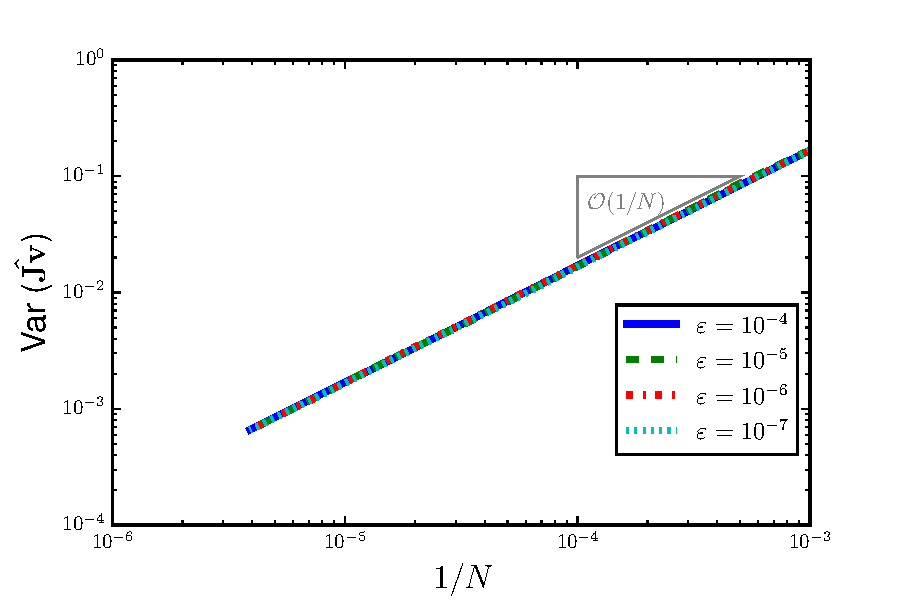
\includegraphics[width=9.5cm]{../Problems/WeightedParticles/checkSystem/plots/Var_N_eps}

\end{frame}





\begin{frame}
\frametitle{Evaluating the bias on Jacobian-vector products}


\begin{equation*} 
 \mathbf{Bias}(\jv, \jvpde ) = \mathbb{\hat{E}}[\jv]  - \jvpde 
\end{equation*}





\pause 

with 
\begin{equation*}
\jvpde \approx \frac{ \U^{\varepsilon}(t + n \Delta t)  - \U (t +  n\Delta t)}{\varepsilon}
\end{equation*}
 \pause 

and $\U$ calculated by explicitly solving 

\begin{equation*}
\label{fokkerplanck}
\pa{\rho(x,t)}{t} + \pa{(a(x) \rho(x,t))}{x} = D  \ppa{\rho(x,t)}{x} 
\end{equation*}

 using

\begin{equation*} 
\rho_i^{n+1} = \rho_i^n + \Delta t \left( \frac{D}{{\Delta x}^2} \left( \rho_{i+1}^{n} - 2 \rho_i^n + \rho_{i-1}^n \right)  - \frac{a(x)}{\Delta x} (\rho_i^n - \rho_{i-1}^n) \right)
\end{equation*}
for the value of $\rho$ at position $x=i \Delta x$ and time $t=(n+1) \Delta t$

\end{frame}

\begin{frame}
\frametitle{Evaluating the bias on Jacobian-vector products}


\begin{equation*} 
 \mathbf{Bias}(\jv, \jvpde ) = \mathbb{\hat{E}}[\jv]  - \jvpde 
\end{equation*}

 
 \begin{figure}
 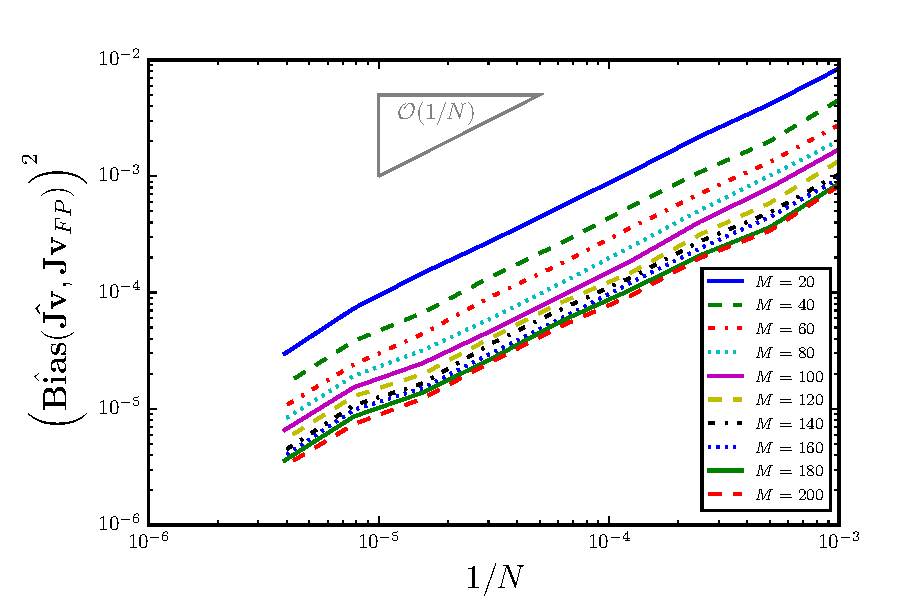
\includegraphics[width=9.5cm]{../Problems/WeightedParticles/checkSystem/plots/Bias_Jv_N_M.pdf}

 \end{figure}

\end{frame}



\begin{frame}
\frametitle{Evaluating the bias on Jacobian-vector products}


\begin{equation*} 
 \mathbf{Bias}(\jv, \jvpde ) = \mathbb{\hat{E}}[\jv]  - \jvpde 
\end{equation*}
 
 \begin{figure}
 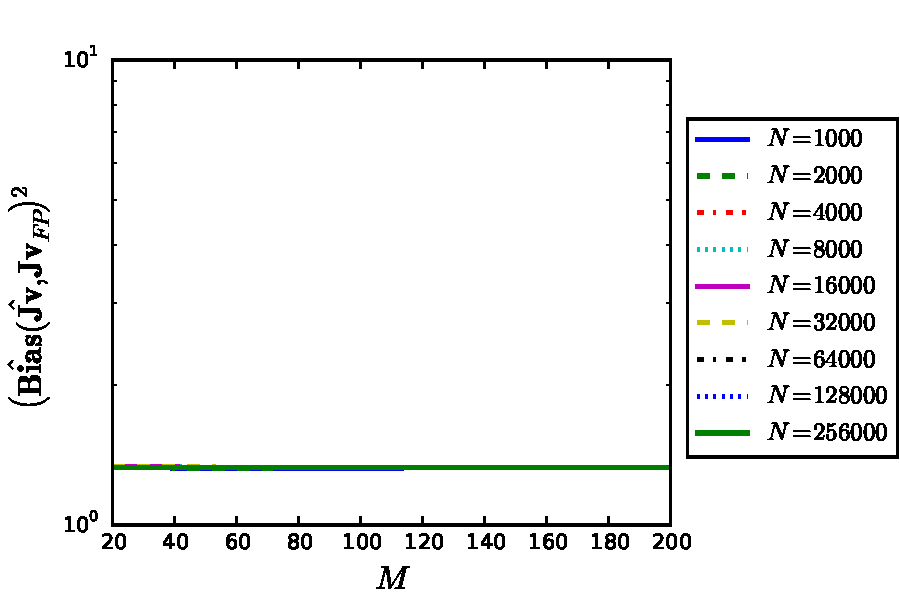
\includegraphics[width=9.5cm]{../Problems/WeightedParticles/checkSystem/plots/Bias_Jv_M_N.pdf}

 \end{figure}

\end{frame}





\end{document}